
\documentclass[12pt, letterpaper]{report}

\title{The Final Report}
\author{Wally Yang, Tina Liang, Wei Zong, Chuwen Sun, Xingyu Yan}
\date{\today}

\usepackage[margin=1in]{geometry}

\usepackage{amsmath}
\setlength{\jot}{12pt} % set the vertical spacing between lines

\usepackage{minted}
\usepackage{xcolor}
\definecolor{monokaibg}{HTML}{272822}

\definecolor{codegreen}{rgb}{0,0.6,0}
\definecolor{codegray}{rgb}{0.5,0.5,0.5}
\definecolor{codepurple}{rgb}{0.58,0,0.82}
\definecolor{backcolour}{rgb}{0.95,0.95,0.92}

\usepackage{amssymb}
\def\ojoin{\setbox0=\hbox{$\bowtie$}%
  \rule[-.02ex]{.25em}{.4pt}\llap{\rule[\ht0]{.25em}{.4pt}}}
\def\leftouterjoin{\mathbin{\ojoin\mkern-5.8mu\bowtie}}
\def\rightouterjoin{\mathbin{\bowtie\mkern-5.8mu\ojoin}}
\def\fullouterjoin{\mathbin{\ojoin\mkern-5.8mu\bowtie\mkern-5.8mu\ojoin}}

\usepackage{graphicx}

\usepackage{multirow}

\begin{document}
\maketitle

\section{Database Description}

\begin{enumerate}
  \item ER-model of the Database Design

    \begin{center}
      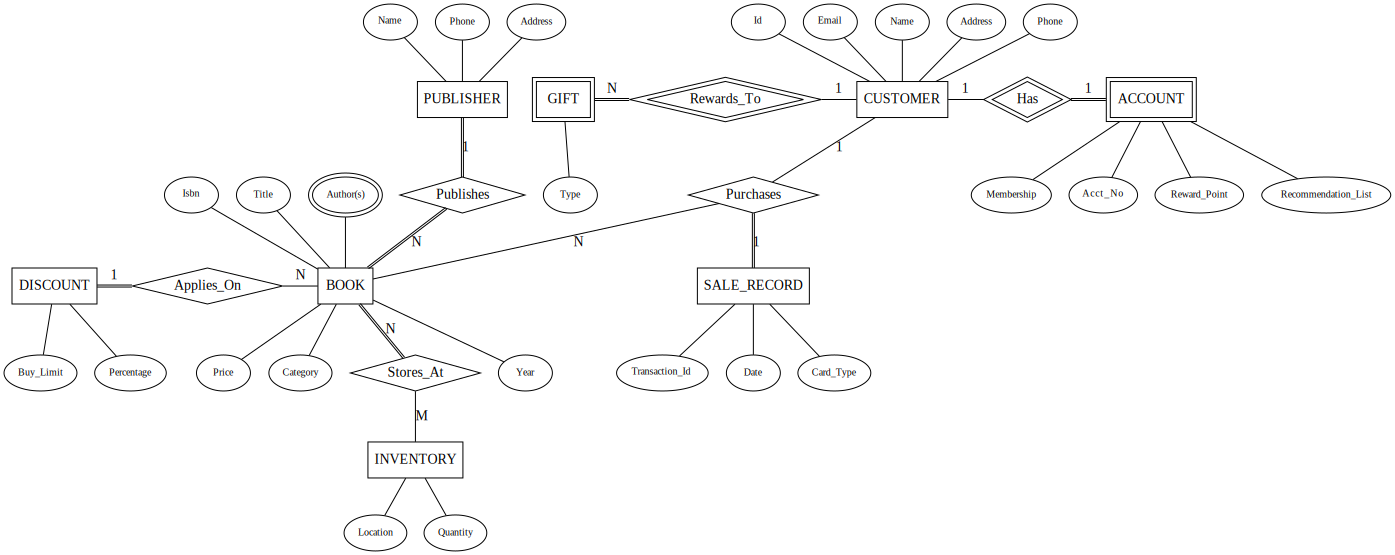
\includegraphics[width=\linewidth]{ER}
    \end{center}

    \pagebreak

  \item Relational Schema for the Database

    \begin{center}
      \includegraphics[width=\linewidth]{RelationalSchema}
    \end{center}

    The bold field refers to the primary keys of the relational schema

  \item Levels of normalization for each table:
    All tables achieve BCNF.

  \item Indices for the Database

    We chose the Tree-based index for our BOOK table since the tree-based index is good for looking up values based on range tests. It will speed up our queries when we want to retrieve the book based on the range of the year or the range of the price. Also it is not too bad for looking up values based on equality tests, so it also can slightly speed up our queries when we are trying to look up books based on the titles, categories, authors, and publishers.

  \item Views for the Database

    \begin{itemize}
    \item View A

      Description: This view is able to show all the titles and their dates of purchase made by each customer. And this could be useful to make book recommendations for a customer by looking at his or her purchase history.

      Relational algebra expression:
      \begin{align*}
        &\textit{R1} \leftarrow \textit{PURCHASE} \bowtie_{\textit{Customer} = \textit{Email}} \textit{Customer}\\
        &\textit{R2} \leftarrow \textit{BOOK} \bowtie_{\textit{Isbn} = \textit{Book}} \textit{R1}\\
        &\textit{Result} \leftarrow \pi_{\textit{Name, Title, Date}}\textit{R2}
      \end{align*}

      \inputminted[
      style=monokai,
      bgcolor=monokaibg,
      linenos]
      {sql}{Section1/view_a.sql}

      Sample output:
      \begin{table}[htbp]
        \centering
        \begin{tabular}{| c | c | c |}
          \hline
          Luqman Finnegan	& OCP:	& 07/01/16\\
          & Oracle9i Certification Kit &\\
          \hline
          Phebe Christian	& SQL Server 2000  & 09/16/18\\
          & for Experienced DBA's &\\
          \hline
          Charlie Dolan	& The Data Warehouse Toolkit: & 07/20/18\\
          & The Complete Guide to Dimensional Modeling &\\
          \hline
          Kiya Mcguire & How To Do Everything with Your Tablet PC	& 01/26/19\\
          \hline
          Amal Terrell & Data Mining: & 06/15/17\\
                 & Practical Machine Learning Tools &\\
                 &and Techniques with Java Implementations &\\
          \hline
        \end{tabular}
      \end{table}

    \item View B

      Description: This view is able to show the total number of books purchased by each customer. And this could be useful to see if this customer deserves a gift by making a certain amount of purchases in this store.

      Relational algebra expression:
      \begin{align*}
        &\textit{R1} \leftarrow \textit{PURCHASE} \bowtie_{\textit{Customer} = \textit{Email}} \textit{Customer}\\
        &\textit{Result} \leftarrow _{\textit{Customer}}\mathcal{F}_{\textit{COUNT Book}}(\textit{R1})
      \end{align*}


      \inputminted[
      style=monokai,
      bgcolor=monokaibg,
      linenos]
      {sql}{Section1/view_b.sql}

      Sample output:
      \begin{table}[htbp]
        \centering
        \begin{tabular}{| c | c |}
          \hline
          Ahmed.12@osu.edu & 1\\
          \hline
          Christian.2@osu.edu	& 1\\
          \hline
          Dolan.3@osu.edu	& 1\\
          \hline
          Finnegan.1@osu.edu	& 1\\
          \hline
          Firth.9@osu.edu	& 1\\
          \hline
        \end{tabular}
      \end{table}

    \end{itemize}

  \item Sample Transactions for the Database

    \begin{itemize}
      \item Transaction A

        Description:
        The customer adds a book to a order and update the book quantity in the inventory

        \inputminted[
        style=monokai,
        bgcolor=monokaibg,
        linenos]
        {sql}{Section1/trans_a.sql}

      \item Transction B

        Description:
        A certain amount(10) of books(Isbn: 616601654) transmitted from one inventory(warehouse) to another(in-sotre)

        \inputminted[
        style=monokai,
        bgcolor=monokaibg,
        linenos]
        {sql}{Section1/trans_b.sql}

      \item Transaction C

        Description:
        Customer redeem 100 reward points to a keychain

        \inputminted[
        style=monokai,
        bgcolor=monokaibg,
        linenos]
        {sql}{Section1/trans_c.sql}

    \end{itemize}

\end{enumerate}

\section{User Manual}
\begin{enumerate}
\item Database Description

  \includegraphics[width=\linewidth]{Section2/description}

\item Sample SQL Queries

  \begin{enumerate}
  \item Find the titles of all books by Pratchett that cost less than \$10

    Return a table that contains the title of that books written by Pratchett and cost less than \$10

  \item Find the titles of all books by Pratchett that cost less than \$10

  \item Find the titles and ISBNs for all books with less than 5 copies in stock

  \item Give all the customers who purchased a book by Pratchett and the titles of Pratchett books they purchased

  \item
  \end{enumerate}
\end{enumerate}

\end{document}